%-------------------------------------------------------------------------------
% GOVERNING EQUATIONS
%-------------------------------------------------------------------------------

\section{Governing Equations} \label{sec:gov_equ}

The following presents an overview of the physical and mathematical framework
for the 2D cavity flow problem introduced in section \ref{sec:driven_cav}. The
aim is to show the theory regarding the Navier-Stokes equations and the
stream-function formulation.

\subsection{Incompressible Navier-Stokes Equations}

An incompressible Newtonian fluid in a domain $\Omega$ is governed by the
Navier-Stokes equations which are,

\begin{align}
\frac{\partial \mathbf{u}}{\partial t} + 
  \mathbf{u} \cdot \nabla \mathbf{u} &= 
  - \frac{1}{\rho} \nabla p + \mu \nabla^2 \mathbf{u} + \mathbf{g},
  \label{eq:ns3d} \\
\nabla \cdot \mathbf{u} &= 0 \label{eq:cont3d},
\end{align}

where $\mathbf{u}$ denotes the velocity vector (2D or 3D). $p$ is the pressure,
$\rho$ is the constant fluid density, $\nu$ is the kinematic viscosity and
$\mathbf{g}$ defines the body acceleration acting on the fluid. The first
equation represents the conservation of momentum, while the second is the
continuity equation. Furthermore, boundary conditions must be applied for these
equations on the domain $\Omega$. \\

For cavity flow problem in a plane, we consider the 2D form of the above
equations without body acceleration. They can be written explicitly for the two
spatial components, 

\begin{align}
\frac{\partial u}{\partial t} + u \frac{\partial u}{\partial x} 
  + v \frac{\partial u}{\partial y} &= 
  - \frac{1}{\rho}\frac{\partial p}{\partial x}
  + \nu \left(\frac{\partial^2 u}{\partial x^2}
  + \frac{\partial^2 u}{\partial y^2}\right) \label{eq:ns2d-u}, \\
\frac{\partial v}{\partial t} + u \frac{\partial v}{\partial x}
  + v \frac{\partial v}{\partial y} &=
  - \frac{1}{\rho}\frac{\partial p}{\partial y} 
  + \nu \left(\frac{\partial^2 v}{\partial x^2}
  + \frac{\partial^2 v}{\partial y^2}\right) \label{eq:ns2d-v}, \\ 
\frac{\partial u}{\partial x}
  + \frac{\partial v}{\partial y} &= 0 \label{eq:cont2d}.
\end{align}

$u$ and $v$ denote the velocities in the $x$ and $y$ directions, respectively.
Equations \eqref{eq:ns2d-u}-\eqref{eq:cont2d} build the underlying framework
for the analysis of the 2D cavity flow.

\subsection{Streamfunction Formulation}

In the case of a 2D incompressible fluid, it is possible to introduce a scalar
function $\Psi(x,y,t)$ called the streamfunction which is defined such that,

\begin{align}
u & = \frac{\partial \Psi}{\partial y}, \label{eq:str_defx} \\
v & = -\frac{\partial \Psi}{\partial x}. \label{eq:str_defy} 
\end{align}

By its definition, the streamfunction satisfies the continuity equation and
therefore the incompressibility condition. Regarding the momentum equations,
the expressions \eqref{eq:str_defx} and \eqref{eq:str_defy} can be used to
obtain a formulation of the Navier-Stokes that only involves the streamfunction
\citep{landau1987}: \todo{pressure is eliminated}

\begin{align}
\partial_t \Delta \Psi = \nu \Delta^2 \Psi
  + (\partial_x \Psi) \partial_y(\Delta \Psi)
  - (\partial_y \Psi) \partial_x(\Delta \Psi). \label{eq:str_dim}
\end{align}

For a shorter notation, the partial derivates of the streamfunction are denoted
as subscripts in the equation above and from now on. \\

It is important to note that $\Psi = constant$ represents the family of curves
of the streamline \citep{landau1987}. Hence, if we know the streamfunction, we
can visualize the streamlines by setting the function to different constant
values.

\subsection{Nondimensionalization}

Viewing a non-dimensional version of the problem is standard to analyze the
cavity flow. Figure \ref{fig:cav_dim} shows the characteristic scales of the 2D
cavity. We will use the same length scale $l$ for both sides of our rectangle,
assuming that the aspect ratio is close to 1. Furthermore, as the magnitude for
our regularized boundary conditions is set to be the same for all lids, we can
use the same velocity scale $U$.

\begin{figure}[h]
  \centering
  \begin{subfigure}[b]{0.42\textwidth}
    \centering
    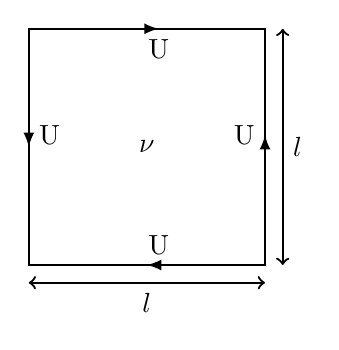
\begin{tikzpicture}[scale=1.5]
      \draw[thick] (0,0) rectangle (2,2);
      \draw[thick] (0,0) rectangle (2,2);

      \node at (1,1) {$\nu$};

      \draw[-latex, thick] (2,0) -- node[pos=0.9, above] {U} (1,0);
      \draw[-latex, thick] (0,2) -- node[pos=0.9, right] {U} (0,1);
      \draw[-latex, thick] (2,0) -- node[pos=1, left] {U} (2,1.1);
      \draw[-latex, thick] (0,2) -- node[pos=1, below] {U} (1.1,2);

      \draw[<->, thick] (0,-0.15) -- node[pos=0.5, below] {$l$} (2,-0.15);
      \draw[<->, thick] (2.15,0) -- node[pos=0.5, right] {$l$} (2.15,2);
    \end{tikzpicture}

    \caption{Characteristic physical dimensions}
    \label{fig:cav_dim}
  \end{subfigure}
  \begin{subfigure}[b]{0.42\textwidth}
    \centering
    \begin{align*}
    \left[ l \right] &= length \\
    \left[ U \right] &= length*time^{-1} \\
    \left[ \Psi \right] &= length^2*time^{-1} \\
    \left[ \frac{l}{U} \right] &= time \quad \text{(dynamic time)} \\
    \end{align*}

    \caption{Scales of the problem}
    \label{eq:scl}
  \end{subfigure}
  \caption{Nondimensional Analysis}
\end{figure}

All parameters can now be made dimensionless by defining $x = l x^*$, $y = l
y^*$, $t = \frac{l}{U} t^*$, $\Psi = lU \Psi^*$. Additionally, the
non-dimensional operators are scaled as $\partial_t = \frac{U}{l}
\partial_{t^*}$, $\partial_x = \frac{1}{l} \partial_{x^*}$, $\partial_y =
\frac{1}{l} \partial_{y^*}$ and $\Delta_* = \frac{1}{l^2} \Delta_{x^*}$. Plugin
these definitions into \eqref{eq:str}, simplifying and dividing by
$\frac{U^2}{L^2}$ we get,

\begin{align*}
\partial_{t^*} \Delta_* \Psi^* = \frac{\nu U}{l} \Delta^2_* \Psi^*
  + (\partial_x^* \Psi^*) \partial_y^*(\Delta_* \Psi^*)
  - (\partial_y^* \Psi^*) \partial_x^*(\Delta_* \Psi^*). 
\end{align*}

We notice that we can recover the Reynolds number $\Rey = \frac{Ul}{\nu}$ that,
as a non-dimensional parameter, characterizes the relative importance of
inertial forces and viscous forces in the flow. For clarity, we will omit ($*$)
notation. All quantities will correspond to the dimensionless variables. The
final equation reads,

\begin{align}
\partial_t \Delta \Psi = \frac{1}{\Rey} \Delta^2 \Psi
  + (\partial_x \Psi) \partial_y(\Delta \Psi)
  - (\partial_y \Psi) \partial_x(\Delta \Psi). \label{eq:str}
\end{align}

This equation will be the foundation for the numerical investigation later on.
The equation is non-dimensional and only depends on the scalar-valued
streamfunction and the Reynolds number. It is a nonlinear ordinary differential
equation of order 4. Different dynamics and regimes can be analyzed by changing
the Reynolds number.

\subsubsection{Scaling the Reynolds number}

As discussed in section \ref{sec:r4sc}, the previous literature has used a
different domain, namely $[0,1] \times [0,1]$ for the four-sided cavity flow.
The reference length $l_{ref}$ used in \citet{wahba2009} and the subsequent
studies is therefor half the length $l$ used here, therefore

\begin{align}
\Rey = \frac{U \cdot l}{\nu} 
  = \frac{sU_{ref} \cdot 2l_{ref}}{\nu} = 2s \cdot \Rey_{ref}.
\end{align}

The scaling factor is $s=\frac{1}{2}$, and the Reynolds number of previous
studies has to be divided by $2$. In all further comparisons of results, the
reference Reynolds numbers of previous works will be scaled to the presented
symmetric domain.
